\documentclass[12pt,english,hyperfootnotes=false,hidelinks]{article}

%%%% Packages
\usepackage{lmodern}
\usepackage{tablefootnote}
\usepackage[T1]{fontenc}
\usepackage[latin9]{inputenc}
\usepackage{geometry}
\geometry{verbose,tmargin=1.25in,bmargin=1.25in,lmargin=1.25in,rmargin=1.25in}
\usepackage{float}
\usepackage{enumitem}
\usepackage{amsmath}
\usepackage{graphicx}
\usepackage{setspace}
\usepackage[authoryear]{natbib}
\usepackage[bottom,multiple]{footmisc}
\usepackage{geometry}
\usepackage{adjustbox}
\usepackage[hyphenbreaks]{breakurl}
\usepackage{booktabs}
\usepackage{pdflscape}
\usepackage{siunitx}
\usepackage{numprint}
\usepackage{threeparttable}
\usepackage{caption}
\usepackage{babel}
\usepackage{xcolor}
\usepackage{longtable}
\usepackage{afterpage}
\usepackage{dcolumn}
\usepackage{multicol}
\usepackage{amsfonts}
\usepackage{adjustbox}
\usepackage{xurl}
\usepackage{hyperref}
\usepackage{catchfilebetweentags}
\usepackage{csquotes}
\usepackage{framed}
\usepackage{multirow}
\usepackage{tikz}
\usetikzlibrary{decorations.pathreplacing}
\usepackage{makecell}
% define check and xmark
\usepackage{pifont}
\newcommand{\cmark}{\ding{51}}%
\newcommand{\xmark}{\ding{55}}%

%%%% Other settings
\captionsetup[table]{skip=0pt}
\interfootnotelinepenalty=10000
\newcolumntype{R}[1]{>{\raggedright\let\newline\\\arraybackslash\hspace{0pt}}m{#1}}
\newcolumntype{C}[1]{>{\centering\arraybackslash}m{#1}}

\newtheorem{assumption}{Assumption}

%%% Command for extracting numbers
\newcommand{\gn}[1]{\ExecuteMetaData[results/results.tex]{#1}}



\title{
Bureaucratic Capacity and Urban Planning: Evidence from Los Angeles
\thanks{
This project was supported in part by the UCLA Ziman Center for Real Estate Research. We thank the Ziman Center for its financial support. We also thank Ignacio Ramirez for his invaluable research assistance. The views expressed in this paper are solely those of the authors and do not necessarily reflect those of the Ziman Center. All errors are our own.
}
}

\author{
    Stuart Gabriel\thanks{UCLA Anderson School of Management, 110 Westwood Plaza, Suite C412, Los Angeles, CA 90095-1481;  stuart.gabriel@anderson.ucla.edu} \and
    Matthew Histen\thanks{California State University, Northridge, David Nazarian College of Business and Economics, 18111 Nordhoff St, Northridge, CA 91330; matthew.histen@csun.edu} \and
    Edward Kung\thanks{Corresponding Author: California State University, Northridge, David Nazarian College of Business and Economics, 18111 Nordoff St, Northridge, CA 91330; edward.kung@csun.edu}
}

\date{\today}

\begin{document}

\maketitle

\singlespacing

\vspace{-1cm}

\begin{abstract}
Lorem ipsum dolor sit amet, consectetur adipiscing elit, sed do eiusmod tempor incididunt ut labore et dolore magna aliqua. Ut enim ad minim veniam, quis nostrud exercitation ullamco laboris nisi ut aliquip ex ea commodo consequat. Duis aute irure dolor in reprehenderit in voluptate velit esse cillum dolore eu fugiat nulla pariatur. Excepteur sint occaecat cupidatat non proident, sunt in culpa qui officia deserunt mollit anim id est laborum.
\end{abstract}


\noindent{\textit{Keywords}: local land-use regulation, bureaucratic efficiency} \\
\noindent {\textit{JEL} Classification: D73, R14, R38, R52.} \\


\doublespacing

\pagebreak


\section{Introduction}\label{sec_intro}

Lorem ipsum dolor sit amet, consectetur adipiscing elit, sed do eiusmod tempor incididunt ut labore et dolore magna aliqua. Ut enim ad minim veniam, quis nostrud exercitation ullamco laboris nisi ut aliquip ex ea commodo consequat. Duis aute irure dolor in reprehenderit in voluptate velit esse cillum dolore eu fugiat nulla pariatur. Excepteur sint occaecat cupidatat non proident, sunt in culpa qui officia deserunt mollit anim id est laborum.
\section{Data}\label{sec_data}

\subsection{Institutional Background}

The Los Angeles planning and approvals process for urban development is a multi-layered process that requires the input of multiple agencies. 


\subsection{Data Acquisition}

The Los Angeles Planning Department's website maintains robust public documentation of City Planning Commission Meetings. For each meeting, the agenda, minutes, and any supplemental documents relevant to the meeting (letters from the public, traffic assessments, architectural reports, etc.) are available for download as PDF files.\footnote{As of August 26th, 2025, these documents are available at the URL: \url{https://planning.lacity.gov/about/commissions-boards-hearings}.} We downloaded these documents for all City Planning Commission meetings from May 10th, 2018 to December 19th, 2024. This resulted in documentary data for \gn{NumberOfMeetings} meetings, covering \gn{NumberOfAgendaItems} agenda items, with \gn{NumberOfSupplementalDocs} supplemental documents, spanning \gn{PageCount} pages of PDF documents. Download occurred on April 10th, 2025.

Since we are primarily interested in bureaucratic decision making, we limit our attention to the agenda items that require a decision from the board. These are identified by agenda items titled according to their Planning Department case numbers, which have a standardized format of ``[CASE PREFIX]-[YEAR]-[SERIAL NUMBER]-[CASE SUFFIXES]''. Other agenda items include items like ``Director's Report'' and ``General Public Comment'' which do not require any decisions on the part of the board. Altogether, there were \gn{NumberOfCases} agenda items requiring a decision from the board, as identified by their Planning Department case numbers.

A typical agenda item is a request from a developer to approve a development plan that goes beyond what the site's zoning designation would allow, or an appeal of a previously approved plan. Figure \ref{fig_example_agenda_item} shows an example of an agenda item. The case number is DIR-2019-6048-TOC-SPR-WDI-1A. This was a project that was initially approved by the Director of Planning (DIR). The project was granted bonuses under the Los Angeles Transit Oriented Communities program (TOC), the project requires a site plan review (SPR), and the project was granted a waiver of dedications and improvements (WDI). However, this previously approved plan was appealed (1A), and the appeal is now to be considered by the City Planning Commission. In addition to the information contained in the case number, the agenda shows additional information such as the Council District that the project is located in, and other specific details about the project proposal.

Figure \ref{fig_example_minutes_item} shows the associated minutes for the agenda item shown in Figure \ref{fig_example_agenda_item}. From the minutes, we can see that the appeal was granted in part and denied in part. The CPC upheld the Director of Planning's previous decision, but additional conditions were applied, thus allowing the project to move forward as long as the developer adheres to the new conditions. This outcome, the partial granting of an appeal or the approval of a project with modifications, is common but not the only kind of outcome. Sometimes, the requested actions by the developer are granted in their entirety without additional conditions or modifications. Rarely, the requested actions are denied entirely. A more common occurrence than denial is that the CPC puts the decision off to a later date. We will discuss the distribution of motion outcomes and voting patterns later in Section \ref{sec_descriptive_statistics}.

Figures \ref{fig_example_support_letter} and \ref{fig_example_oppose_letter} show examples of letters submitted by the public in support of and in opposition to the above project. The support letter emphasizes how the project will ease traffic, reduce air pollution, and increase housing availability. The opposition letter emphasizes concerns about displacement and how the proposed units will be unaffordable to current residents of the neighborhood. These letters typify the kinds of concern expressed by community residents in this dataset; however, the number of letters that this project attracted is atypical (DIR-2019-6048 just happens to be a particularly controversial project). We will discuss the distribution of support and opposition letters across projects later in Section \ref{sec_descriptive_statistics}.

\subsection{Data Extraction}

The documentary data provides a wealth of information about CPC cases and their outcomes. However, the information is locked within textual data that is difficult to process using traditional methods. For example, traditional NLP methods based on token and pattern matching would have a hard time comparing the agenda to the minutes and determining whether the requested actions were approved, partially approved, approved with conditions, denied, or whether the decision was postponed to a future date. 

To extract usable features from the textual content more robustly, we make use of OpenAI's \texttt{gpt-4o} generative language model. For example, the model can be asked to read the text of the agenda, read the text of the minutes, and explain what the result of committee's proposed motion was in terms of its implications for the development project---was the project approved, partially approved or approved with conditions, denied, or was the decision postponed? The methodology and prompts we used to perform the data extraction are described in detail in Appendix \ref{sec_data_appendix}. In this section, we will instead focus on the data features that were extracted from the text.

\paragraph{Agenda items.} For each agenda item, we extracted the following information from the text: 
\begin{itemize}[noitemsep, topsep=0pt]
\item Item number (used primarily for identification);
\item Item title (for cases requiring a decision, this is always a Planning Department case number)
\item Short AI-generated summary of the agenda item's content;
\item The Council District(s) to which the item applies
\end{itemize}

\paragraph{Minutes.} For each agenda item, we extract the following information from its minutes text:
\begin{itemize}[noitemsep, topsep=0pt]
\item Short AI-generated summary of the deliberations and the motion that was ultimately voted on;
\item Implication of the motion for the proposed project: were the requested actions approved, approved in part or with conditions and modifications, denied, or were deliberations continued to a future date?
\item Result of the vote (whether the motion passed or failed)\footnote{Note that a motion passing is not the same as a project getting approved, nor is a motion failing the same as a project getting denied. A Member may move to deny the project's requested actions, or move to accept an appeal of a previously approved project, in which case the motion passing implies a denial of the project. These nuances highlight why LLMs are helpful in the data extraction process.};
\item Vote tallies: the number of ayes, nays, absences, abstentions, and recusals.
\end{itemize}

\paragraph{Supplemental documents.} For each supplemental document, we extract the following information from its text:
\begin{itemize}[noitemsep, topsep=0pt]
\item Type of document: whether it is a letter or petition, a technical modification or procedural matter, a scientific or technical report (traffic, environmental, etc), or a credentials document (CV, resume, biography, etc); 
\item Type of author: whether the author of the document is an individual, an advocacy group, a consultant, a lawyer, a developer, or a public official;
\item Which agenda item(s) it references;
\item Short AI-generated summary of the document contents;
\item Support or opposition: Whether the document definitely supports, somewhat supports, is neutral towards, somewhat opposes, or definitely opposes the referenced agenda item(s).
\end{itemize}

~

\noindent The resulting dataset contains \gn{NumberOfCases} agenda items with motions voted on by the CPC. Table \ref{tab_result_unanimity} shows the distribution of the motion outcomes by the unanimity of the vote. Two important facts emerge about the CPC process. First, a minuscule number of projects are denied outright (\gn{CasesDeniedPct} of all cases). Rather than being denied, a more common occurrence is that the decision is postponed to a later date (\gn{CasesContinuedPct} of cases) or the requested actions are only partially approved or approved with conditions or modifications (\gn{CasesApprovedWithModsPct} of cases). Second, most decisions were unanimous (\gn{CasesUnanimousPct} of all cases). Because of these two facts, we do not view disagreement \emph{within} the board as a significant source of friction in moving development projects through the pipeline. Moreover, few projects are denied outright, so the impact of CPC hearings on final outcomes must come through either i) a slowing down of the process due to having to wait for the decision, which itself may be delayed multiple times; or ii) changes to the project plan that potentially add cost or time to the development, or which could  dissuade the developer from even moving forward with the project. Our primary analysis will therefore focus on the bureaucratic factors which lead to either delayed decision making or attaching conditions and modifications to the project proposal.



\section{Methodology}\label{sec_methodology}

We model the CPC hearings as having three possible outcomes:
\begin{enumerate}[start=0]
\item The project is denied or the decision is postponed;
\item The project is approved in part or with conditions or modifications;
\item The project is approved.
\end{enumerate}
Each project proposal $i$ is assumed to have a latent quality variable $y_i^\ast$ which determines the likelihood of the three outcomes. $y_i^\ast$ is modeled as a linear function of its observed project characteristics and bureaucratic factors, $\mathbf{X}_i$, plus an error term $\epsilon_i$:
\begin{align}
y_i^\ast = \mathbf{X}_i \beta + \epsilon_i
\end{align}
The latent quality of the project proposal determines its outcome at the CPC hearing. Let $y_{i} \in \{0, 1, 2\}$ denote project $i$'s outcome. The relationship between $y_i^\ast$ and $y_i$ is as follows:
\begin{align}
y_i = \begin{cases}
0 \text{ if } y_i^\ast < \mu_0 \\
1 \text{ if } \mu_0 \leq y_i^\ast < \mu_1 \\
2 \text{ if } \mu_1 \leq y_i^\ast
\end{cases}
\end{align}
with $\mu_0 < \mu_1$. The model is therefore an ordered logit model, and the outcomes are monotonic in $\mathbf{X}_i \beta$. The parameters $\beta$, $\mu_0$, and $\mu_1$ are estimated by maximum likelihood.

\subsection{Explanatory Variables}

We now turn to discussing the explanatory variables we include in the model.

\paragraph{Semantic uniqueness.} In that one of our goals is to quantify the role of bureaucratic frictions in the CPC approvals process, we here develop a concept which we call ``semantic uniqueness''. At a high level, semantic uniqueness is designed to capture how unique an agenda item is relative to other agenda items that the CPC is accustomed to facing. Our hypothesis is that agenda items which are highly unusual may be less likely to be approved, and more likely to be approved with conditions or denied or delayed. We thus expect to estimate a negative coefficient on semantic uniqueness.

To compute a measure of semantic uniqueness, we first calculate the semantic embedding of each agenda item using OpenAI's \texttt{text-embedding-3-small} embeddings model.\footnote{For an introduction to the concept of embeddings, see \citet{mikolov2013} and \citet{le2014}.} For each agenda item, the model returns a 1,536 dimensional numerical vector that represents the semantic meaning of the text. Two agenda items with very similar proposals will have embeddings that are close to each other, while two agenda items with very different proposals will have embeddings that are far away from each other. 

Because \texttt{text-embedding-3-small} was trained on a general corpus of documents, not specialized to the topic of municipal planning and zoning, not all 1,536 dimensions may be relevant for capturing the important differences between our agenda items. We therefore use principal components analysis to extract the 10 linear combinations of these dimensions which explain the most variance in our corpus. Figure \ref{fig_scree_plot} shows the scree plot of the principal components analysis. By the 10th principal component, there are diminishing returns to including more components.

After reducing the embeddings down to 10 dimensions, we group the agenda items into three clusters using K-Means clustering. Identifying clusters in our data is important because the CPC handles many different types of cases, and the language used could be quite different across cases of differing types. For example, the language used in a case involving the demolition of a building followed by reconstruction of a multifamily building would be very different from the language used in a case involving the conditional use permit to operate a school. Thus, it only makes sense to measure semantic uniqueness within a set of cases of similar type.

Figure \ref{fig_clusters} shows a scatter plot of the agenda items according to their first two principal components, colored by cluster. Cluster 0, the largest cluster, consists mainly of proposals to build new buildings. Cluster 1 consists mainly of citywide code amendments and general or community plan updates that the CPC must approve. Cluster 2, the smallest cluster, consists primarily of conditional use permits (requests to utilize facilities for purposes not allowed by right within the zoning designation.)

To measure the semantic uniqueness of an agenda item, we calculate the Mahalanobis distance between the agenda item's 10-dimensional PCA-reduced embedding to its cluster's centroid. We chose the Mahalanobis distance because [Joe explain]. In the regressions, we normalize the measured semantic uniqueness to have mean 0 and a variance of 1 across all our agenda items.

In addition to including the Mahalanobis distance to the cluster centroid as a measure of semantic uniqueness, we also include fixed effects for each cluster. This allows each cluster to have a separate baseline probability distribution over outcomes.

\paragraph{Perplexity.} Semantic uniqueness measures how unusual a proposal is relative to other cases of similar type. In addition to that, we also try to measure how confusing or hard to understand a proposal is in general. To do this, we ask \texttt{gpt-4o} to summarize each agenda item, then we measure the perplexity of the response. In language models, perplexity is a measure of how uncertain the model is about its response. It is measured as the exponent of the response's cross-entropy  (i.e. the negative mean of the output tokens' conditional log probabilities.)\footnote{See \citet{jm2}.} A perplexity of 1 indicates that the model has no uncertainty about its output, while a higher perplexity means the model is more uncertain. As with semantic uniqueness, we normalize perplexity to have a mean of 0 and a variance of 1 before including it in the regressions.

\paragraph{Agenda order.} We also hypothesize that the order in which a case appears in the agenda may matter for its outcome. Note that we use the order in which the case appears in the agenda, not the order in which the case was discussed at the actual meeting. The committee chair has the ability to discuss agenda items out of order, and this may be endogenous to the meeting outcomes, so we focus on the order in which the item appears in the agenda published prior to the start of the meeting.

\paragraph{Number of agenda items.} We hypothesize that the number of items on the agenda can have an effect on outcomes. In particular, we hypothesize that a case is more likely to be postponed if there are a large number of items on the agenda.

\paragraph{Consent calendar.} The Los Angeles CPC utilizes a practice for streamlining meetings known as the ``consent calendar''. The consent calendar takes multiple agenda items and groups them into a single motion that the committee votes on together as a whole. The consent calendar tends to include cases that the committee chair has deemed non-controversial and therefore not requiring separate discussion. The consent calendar is published \emph{before} the meeting starts, and items can be taken off the consent calendar during the meeting. We hypothesize that being on the consent calendar before the meeting starts significantly predicts approval.

\paragraph{Number of support and opposition letters.} We hypothesize that the amount of public support or public opposition matters for hearing outcomes. We hypothesize that more public support improves a proposal's probability of being approved, while more public opposition increases the likelihood that the proposal is denied, delayed, or approved with modifications. We public support and public opposition as two separate explanatory variables to allow for heterogeneous impacts of support vs. opposition. We measure public support as the log base 2 of the number of letters written in support, and we measure public opposition as the log base 2 of the number of letters written in opposition, as discussed in Section \ref{sec_data}. 

\paragraph{Council districts.} Council districts may matter for case outcomes for a variety of reasons. For one, although City Planning Commission members are appointed from a variety of professional backgrounds, most of them come from backgrounds of urban planning, public service, real estate development, or community advocacy. In all these cases, the member, despite best efforts to remain impartial, may still be influenced by the specific politics of the council district. For another, the Los Angeles City Council has veto power over City Planning Commission decisions, and in such decisions the council members usually defer to the opinion of the member in charge of the district that the project is located in. The CPC's decisions on a project could therefore be influenced by the opinions of the City Council member in charge of the district the project is located in. To control for these possibilities, we include council district fixed effects as explanatory variables.

\paragraph{Case suffixes.} As discussed in Section \ref{sec_data}, case suffixes indicate the types of entitlements requested or required by the project. In the raw dataset, there were over 70 unique case suffixes, which is too many dummy variables to include in a dataset with only \gn{NumberOfCases} observations. We therefore group the suffixes into XX groups, and include fixed effects for each of these suffix groups. The suffix groups are as follows:
\begin{enumerate}
\item suffix group 1
\item suffix group 2
\end{enumerate}
[Joe fill out]










\section{Results}\label{sec_results}

Here are the results.


\section{Conclusion}\label{sec_conclusion}

And now the conclusion.

%\bibliographystyle{aer}
%\bibliography{81refs}

%\pagebreak

\pagebreak

\begin{figure}[H]
\caption{Example of an Agenda Item} \label{fig_example_agenda_item}
\vspace{-0.5cm}
\begin{center}
\fbox{
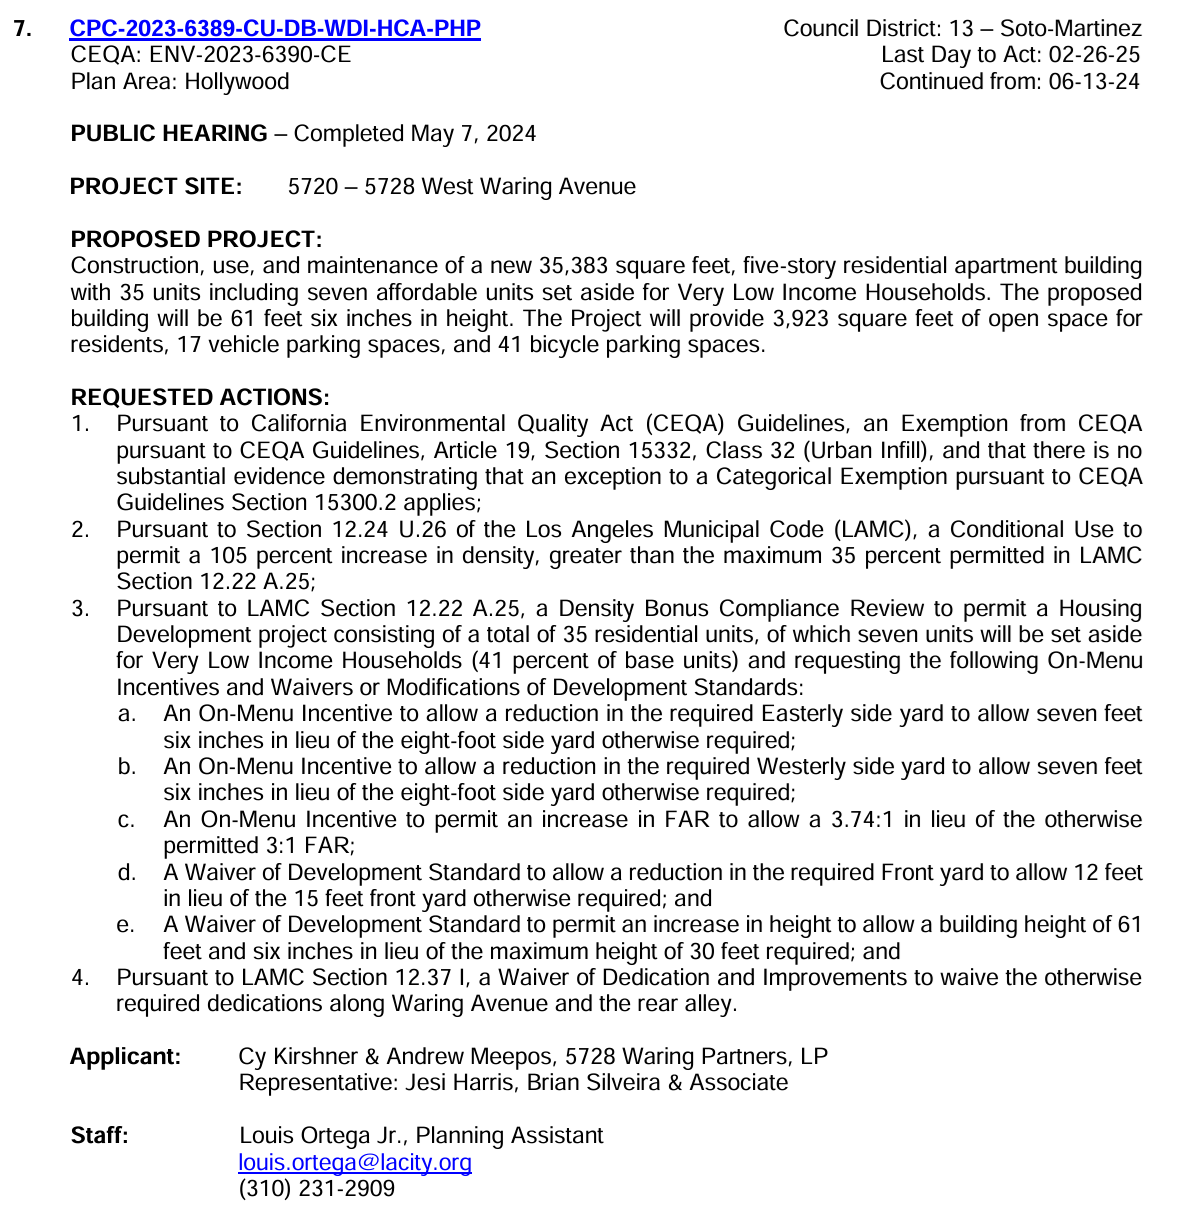
\includegraphics[width=\textwidth]{figures/example-agenda-item.png}
}
\end{center}
\end{figure}

\pagebreak

\begin{figure}[H]
\caption{Example of a Minutes Item} \label{fig_example_minutes_item}
\vspace{-0.5cm}
\begin{center}
\fbox{
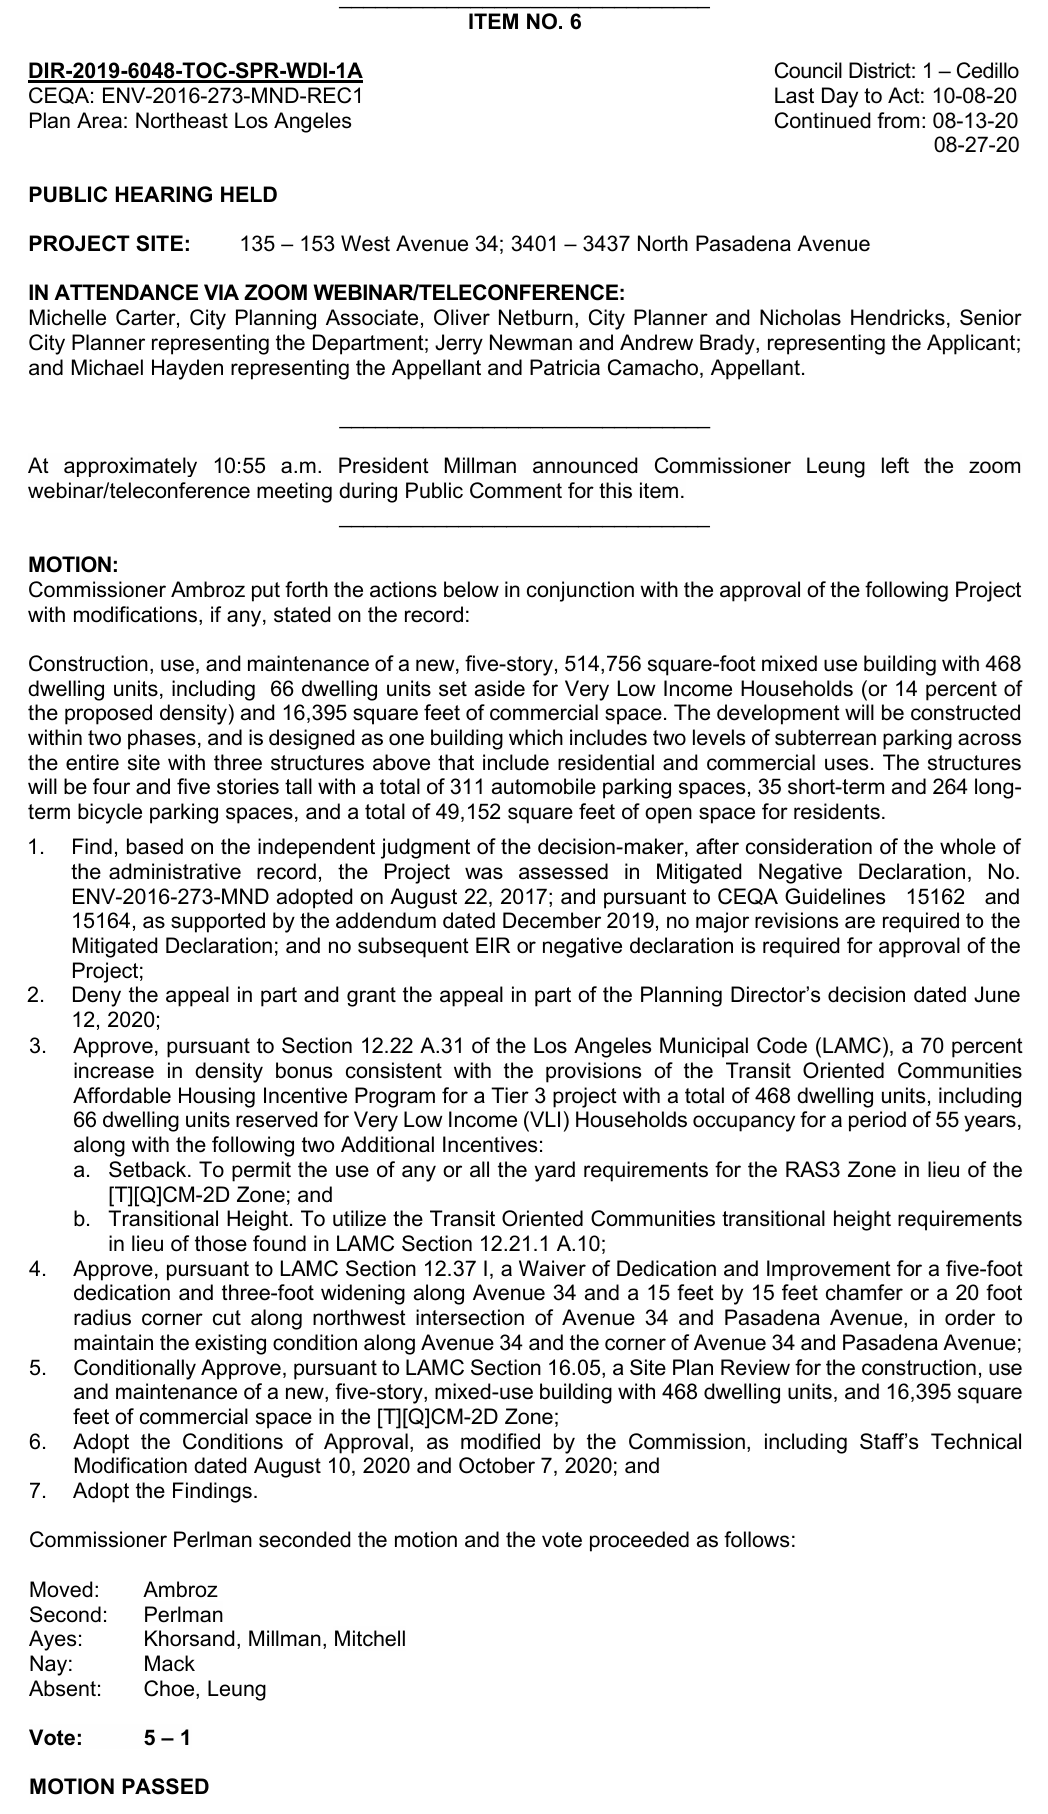
\includegraphics[height=0.95\textheight]{figures/example-minutes-item.png}
}
\end{center}
\end{figure}

\pagebreak

\begin{figure}[H]
\caption{Example of a Support Letter} \label{fig_example_support_letter}
\vspace{-0.5cm}
\begin{center}
\fbox{
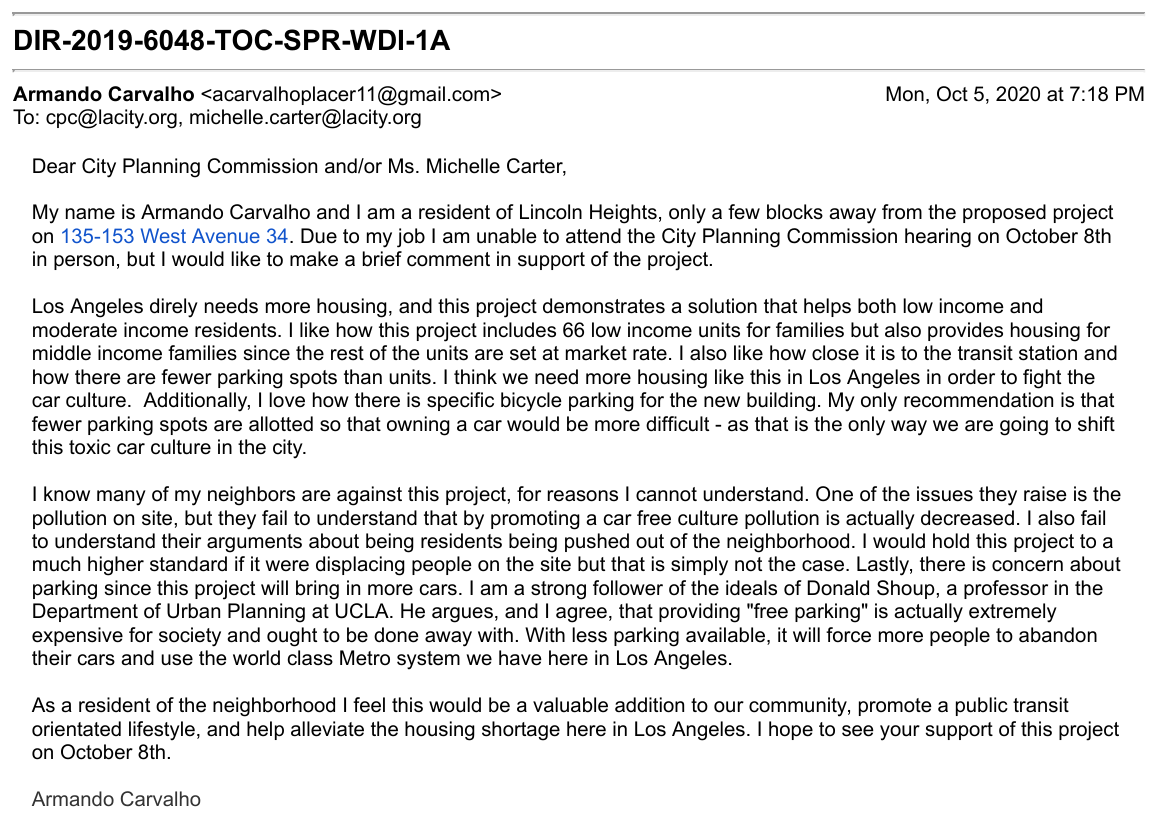
\includegraphics[width=\textwidth]{figures/example-support-letter.png}
}
\end{center}
\end{figure}

\pagebreak

\begin{figure}[H]
\caption{Example of an Oppose Letter} \label{fig_example_oppose_letter}
\vspace{-0.5cm}
\begin{center}
\fbox{
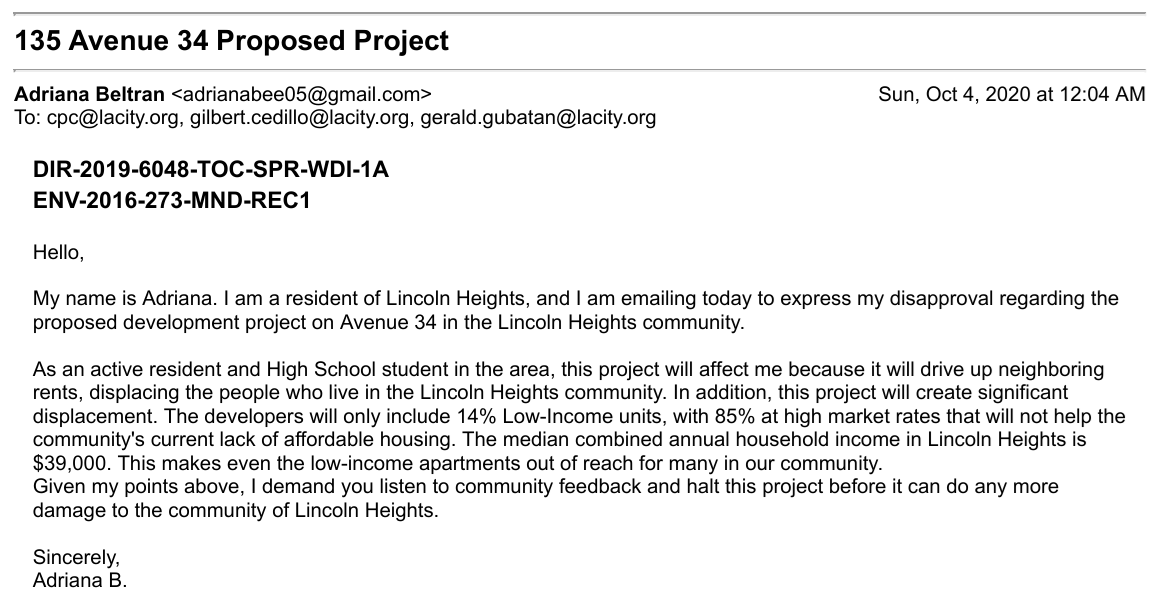
\includegraphics[width=\textwidth]{figures/example-oppose-letter.png}
}
\end{center}
\end{figure}

\pagebreak

\begin{table}[H]
\caption{Summary of Motion Outcomes and Vote Results}
\vspace{0.2cm}
\label{tab_result_unanimity}
\begin{adjustbox}{max width=\textwidth}
\begin{threeparttable}
\begin{tabular}{lrrrrr} \toprule
 & \multicolumn{3}{c}{Unanimity} &  & \\ \cline{2-4} 
 & Unanimous & 1 Nay & >1 Nays & \multicolumn{2}{c}{Total} \\ \midrule
\textit{Project Implication} & & & & & \\ 
~ ~ APPROVED & 365 & 23 & 4 & 392 & (53.9\%) \\ [1ex] 
~ ~ APPROVED IN PART OR WITH MODIFICATIONS & 183 & 17 & 16 & 216 & (29.7\%) \\ [1ex] 
~ ~ DELIBERATIONS CONTINUED TO FUTURE DATE & 108 & 4 & 0 & 112 & (15.4\%) \\ [1ex] 
~ ~ DENIED & 5 & 0 & 2 & 7 & (1.0\%) \\ [1ex] 
~ ~ TOTAL & 661 & 44 & 22 & 727 &  \\ [1ex] 
 & (90.9\%) & (6.1\%) & (3.0\%) &  &  \\ [1ex] 
\end{tabular}

\begin{tablenotes}

\item {\textit{Notes: } This table shows the number of cases decided on by the City Planning Commission, organized by the implication of the motion for the project proposal and the unanimity of the vote.}
\end{tablenotes}
\end{threeparttable}
\end{adjustbox}
\end{table}

\pagebreak

\begin{table}[H]
\caption{Summary Statistics for Case Features}
\vspace{0.2cm}
\label{tab_summary_stats}
\begin{adjustbox}{max width=\textwidth}
\begin{threeparttable}
\begin{center}
[Summary statistics for variables used in analysis]
\end{center}
\begin{tablenotes}
\item {\textit{Notes: } Notes.}
\end{tablenotes}
\end{threeparttable}
\end{adjustbox}
\end{table}

\pagebreak

\begin{table}[H]
  \caption{Ordered Logit Regression Results}
  \vspace{0.2cm}
  \label{tab_ologit_results}
  \begin{adjustbox}{max width=\textwidth}
    \begin{threeparttable}
      \centering
      \begin{tabular}{lcccc}
\toprule
 & (1) & (2) & (3) & (4) \\
\midrule
 &  &  &  &  \\
Semantic Uniqueness & -0.325*** & -0.258*** & -0.259*** & -0.228** \\
 & (0.080) & (0.083) & (0.088) & (0.105) \\
 &  &  &  &  \\
Agenda Perplexity &  & -4.649 & -3.548 & -3.861 \\
 &  & (3.209) & (3.197) & (3.250) \\
 &  &  &  &  \\
Agenda Order &  & 0.095* & 0.086* & 0.042 \\
 &  & (0.050) & (0.050) & (0.053) \\
 &  &  &  &  \\
No. Agenda Items &  & -0.053 & -0.041 & -0.013 \\
 &  & (0.044) & (0.044) & (0.046) \\
 &  &  &  &  \\
Consent Calendar &  & 1.456*** & 1.357*** & 1.423*** \\
 &  & (0.279) & (0.292) & (0.304) \\
 &  &  &  &  \\
$\log_2$(\# Support) &  & 0.038 & 0.049 & 0.051 \\
 &  & (0.055) & (0.058) & (0.057) \\
 &  &  &  &  \\
$\log_2$(\# Oppose) &  & -0.169*** & -0.195*** & -0.209*** \\
 &  & (0.054) & (0.058) & (0.059) \\
 &  &  &  &  \\
Semantic Cluster FE & N & Y & Y & Y \\
 &  &  &  &  \\
Council District FE & N & N & Y & Y \\
 &  &  &  &  \\
Suffix Group FE & N & N & N & Y \\
 &  &  &  &  \\
$\mu_0$ & -2.641*** & -7.425** & -6.324* & -6.248* \\
 & (0.271) & (3.516) & (3.520) & (3.563) \\
 &  &  &  &  \\
$\mu_1$ & -1.136*** & -5.844* & -4.696 & -4.556 \\
 & (0.253) & (3.504) & (3.505) & (3.549) \\
 &  &  &  &  \\
No. of Obs & 727 & 727 & 727 & 727 \\
Pseudo R2 & 0.013 & 0.049 & 0.068 & 0.090 \\
\bottomrule
\end{tabular}

\begin{tablenotes}[flushleft]
        \footnotesize
        \item Robust standard errors in parentheses; * $p<0.05$, ** $p<0.01$, *** $p<0.001$.
        \item \textit{Notes:} This table reports results from the ordered logit regression 
        discussed in Section \ref{sec_methodology}. The ordering of the outcomes is 
        0: DENIED / DELIBERATIONS CONTINUED TO FUTURE DATE; 
        1: PARTIALLY APPROVED OR APPROVED WITH MODIFICATIONS; 
        2: APPROVED.
      \end{tablenotes}
    \end{threeparttable}
  \end{adjustbox}
\end{table}



\pagebreak

\appendix

\renewcommand{\thefigure}{\thesection\arabic{figure}}
\renewcommand{\thetable}{\thesection\arabic{table}}

\makeatletter
\@addtoreset{figure}{section}
\@addtoreset{table}{section}
\makeatother

\section{Data Appendix} \label{sec_data_appendix}

\subsection{Data Extraction with LLMs}

Extracting data from the raw PDFs downloaded from the Planning Department website is a multi-step process. First, individual agenda items need to be extracted from the raw agenda PDF. This is difficult using traditional NLP methods because the boundaries between agenda items in the PDF are not always consistently demarcated. However, LLMs are quite suited to this task of identifying the unique agenda items out of a single PDF containing the agenda.

The first step, therefore, is to extract the individual agenda items. Figure \ref{fig_split_agenda_prompt} shows the prompt we used to have the LLM read the agenda, then extract each individual agenda item. We ask the LLM to return the agenda's item number, its title (which is a Planning Department case number for any items requiring a decision), and a short summary of the agenda item.

After the agenda items are extracted, the next step is to extract data about each agenda item, using the agenda text. The raw agenda PDF is split into its individual components based on the extracted item number and title for each agenda item. The text for each individual agenda item is then fed into the prompt shown in Figure \ref{fig_agenda_items_prompt}. The outputted response is then used to extract the data features listed in Section \ref{sec_data}.

After extracting data from the agenda text, we extract information about the deliberations over each agenda item from the minutes text. We first split the minutes PDF into the components relevant to each individual item, using the item number and title. We then take the agenda text for that item and the minutes text for that item and feed it into the prompt shown in Figure \ref{fig_minutes_prompt}. The response from the LLM is then processed to extract the data features.

Lastly, we 



\pagebreak

\begin{figure}[H]
\caption{Prompt to Split and Summarize Agenda} \label{fig_split_agenda_prompt}
\vspace{-0.5cm}
\begin{center}
\fbox{
\begin{minipage}{\textwidth}
\texttt{
\footnotesize
The following extracted PDF text contains the agenda for a LA City Planning Commission meeting. \\ 
\\ 
For each agenda item, return a summary in the following format:\\ 
\\ 
ITEM NO: <agenda item number>\\ 
TITLE: <title of agenda item>\\ 
SUMMARY: <short summary of agenda item>\\ 
\\ 
Separate each response by "------"\\ 
\\ 
AGENDA:\\ 
\\ 
[AGENDA TEXT]
}
\end{minipage}
}
\end{center}
\end{figure}

\pagebreak

\begin{figure}[H]
\caption{Prompt to Extract Agenda Item Data} \label{fig_agenda_items_prompt}
\vspace{-0.6cm}
\begin{center}
\fbox{
\begin{minipage}{\textwidth}
\texttt{
\footnotesize
--- AGENDA ITEM ----\\ 
\\ 
<<agenda item text>>\\ 
\\ 
--- PROMPT ----\\ 
\\ 
The document above is an agenda item from a Los Angeles City Planning Commission (CPC) meeting.\\ 
\\ 
Please return a response in the following format:\\ 
\\ 
---- YOUR RESPONSE FORMAT ----\\ 
RELATED CASES:\\ 
<A comma separated list of relevant planning department case numbers>\\ 
\\ 
COUNCIL DISTRICT:\\ 
<What council district is the project located in? Your only options are: 1, 2, 3, 4, 5, 6, 7, 8, 9, 10, 11, 12, 13, 14, 15, CITYWIDE>\\ 
\\ 
COUNCIL MEMBER:\\ 
<Who is the council member representing that district? If district is CITYWIDE, say N/A>\\ 
\\ 
LAST DAY TO ACT:\\ 
<What is the last day to act? Format your answer as YYYY-MM-DD>\\ 
\\ 
SUMMARY OF PROJECT:\\ 
<Summarize the project and the requested actions.>\\ 
\\ 
RELEVANT LAWS:\\ 
<List any referenced legal codes, ordinances, or programs that apply to the requested actions>\\ 
\\ 
APPEALED:\\ 
<Was there an appeal against an earlier determination? Say YES or NO>\\ 
\\ 
SUMMARY OF APPEAL:\\ 
<Summarize the appeal if there was one. If no appeal, say N/A>\\ 
\\ 
DISPUTED LAWS:\\ 
<List the referenced legal codes, ordinances, or programs which are in dispute based on the appeal. If no appeal, say N/A>
}
\end{minipage}
}
\end{center}
\end{figure}

\pagebreak

\begin{figure}[H]
\caption{Prompt to Extract Data from Minutes} \label{fig_minutes_prompt}
\vspace{-0.6cm}
\begin{center}
\fbox{
\begin{minipage}{\textwidth}
\texttt{
\footnotesize
--- AGENDA ITEM ----\\ 
\\ 
<<agenda item text>>\\ 
\\ 
--- MINUTES OF DISCUSSION ----\\ 
\\ 
<<minutes text for item>>\\ 
\\ 
--- PROMPT ----\\ 
\\ 
I just gave you two documents related to a Los Angeles City Planning Commission (CPC) hearing.\\ 
\\ 
The first document is the agenda item to be discussed, with requested actions.\\ 
\\ 
The second document is the minutes of the discussion, the proposed motion by the CPC, the votes on the motion by the CPC members, and whether the motion ultimately passed.\\ 
\\ 
Please return a response in the following format:\\ 
\\ 
---- YOUR RESPONSE FORMAT ----\\ 
RELATED CASES:\\ 
<A comma separated list of relevant planning department case numbers>\\ 
\\ 
SUMMARY OF AGENDA ITEM:\\ 
<A summary of the agenda item to be discussed>\\ 
\\ 
SUMMARY OF CPC DELIBERATIONS:\\ 
<A summary of the deliberations of the CPC.>\\ 
\\ 
SUMMARY OF CPC MOTION:\\ 
<A summary of the motion voted on by the CPC>\\ 
\\ 
MOVED:\\ 
<Which commission member moved the motion? If multiple motions were made, use only the last motion. If no motion was made, say "N/A".>\\ 
\\ 
SECONDED:\\ 
<Which commission member seconded the motion? If multiple motions were made, use only the last motion. If no motion was made, say "N/A".>
}
\end{minipage}
}
\end{center}
\end{figure}

\pagebreak

\begin{figure}[H]\ContinuedFloat
\caption{Prompt to Extract Data from Minutes (cont'd)} \vspace{-0.6cm}
\begin{center}
\fbox{
\begin{minipage}{\textwidth}
\texttt{
\footnotesize
AYES:\\ 
<A comma separated list of commission members who voted for the motion. If multiple motions were made, use only the last motion. If no one voted for, say "NONE". If no motion was made, say "N/A".>\\ 
\\ 
NAYS:\\ 
<A comma separated list of commission members who voted against the motion. If multiple motions were made, use only the last motion. If no one voted against, say "NONE". If no motion was made, say "N/A".>\\ 
\\ 
ABSTAINED:\\ 
<A comma separated list of commission members who abstained from voting on the motion. If multiple motions were made, use only the last motion. If no one abstained, say "NONE". If no motion was made, say "N/A".>\\ 
\\ 
RECUSED:\\ 
<A comma separated list of commission members who were recused from voting on the motion. If multiple motions were made, use only the last motion. If no one was recused, say "NONE". If no motion was made, say "N/A".>\\ 
\\ 
ABSENT:\\ 
<A comma separated list of commission members who were absent. If multiple motions were made, use only the last motion. If no one was absent, say "NONE". If no motion was made, say "N/A".>\\ 
\\ 
VOTE RESULT:\\ 
<Did the motion pass or fail? Your only options are MOTION PASSED, MOTION FAILED, N/A>\\ 
\\ 
RESULT OF APPEAL:\\ 
<If the agenda item involved an appeal, say whether the appeal was granted or denied. Your only options are: APPEAL GRANTED, APPEAL GRANTED IN PART, APPEAL DENIED, NO APPEAL, DELIBERATIONS CONTINUED TO FUTURE DATE, APPLICATION WITHDRAWN>\\ 
\\ 
IMPLICATION FOR PROJECT:\\ 
<What is the implication of the vote for the original requested actions? Your only options are: APPROVED, APPROVED IN PART OR WITH MODIFICATIONS, DENIED, DELIBERATIONS CONTINUED TO FUTURE DATE, APPLICATION WITHDRAWN>
}
\end{minipage}
}
\end{center}
\end{figure}

\pagebreak

\begin{figure}[H]
\caption{Prompt to Extract Data from Supplemental Documents} \label{fig_supplemental_docs_prompt}
\vspace{-0.6cm}
\begin{center}
\fbox{
\begin{minipage}{\textwidth}
\texttt{
\footnotesize
==== LIST OF AGENDA ITEMS ====\\ 
\\ 
<<full agenda text>>\\ 
\\ 
==== DOCUMENT ====\\ 
\\ 
<<document text>>\\ 
\\ 
==== PROMPT ====\\ 
\\ 
I just gave you a list of agenda items from a LA City Planning Commission meeting, followed by a document submitted to that meeting. \\ 
\\ 
Return a response in the following format:\\ 
\\ 
\\ 
==== YOUR RESPONSE FORMAT ====\\ 
\\ 
TYPE OF DOCUMENT:\\ 
<What type of document is it? Your only options are: LETTER OR PETITION, TECHNICAL MODIFICATION OR PROCEDURAL MATTER, SCIENTIFIC OR TECHNICAL REPORT, CV OR BIOGRAPHY, CORRUPTED/ILLEGIBLE/BLANK, TITLE OR SECTION HEADING, OTHER.>\\ 
\\ 
TYPE OF AUTHOR:\\ 
<What type of entity wrote the document? Your only options are: INDIVIDUAL, ADVOCACY GROUP, CONSULTANT, LAWYER, DEVELOPER, PUBLIC OFFICIAL, OTHER.>\\ 
\\ 
SUMMARY OF DOCUMENT:\\ 
<Summarize the contents of the document.>\\ 
\\ 
REFERENCED AGENDA ITEMS:\\ 
<List the agenda items, as a comma delimited list of item numbers, that the submitted document references or is relevant to. If none, say NONE.>\\ 
\\ 
SUPPORT OR OPPOSE:\\ 
<Does the submitted document support or oppose the referenced agenda items? Your only options are: DEFINITELY SUPPORT, SOMEWHAT SUPPORT, DEFINITELY OPPOSE, SOMEWHAT OPPOSE, NEUTRAL, NOT RELEVANT.>
}
\end{minipage}
}
\end{center}
\end{figure}


\end{document}

